\section{Hintergrund}

Die vorliegende Bachelorarbeit hat zum Ziel, die Robotersteuerungssoftware, die
derzeit auf Micro-ROS basiert, auf FreeRTOS zu portieren, um einen
vergleichenden Leistungsanalyse zwischen beiden Plattformen durchzuführen. Beide
Systeme sind für die Steuerung eines mobilen Roboters auf einem Cortex-M7
Mikrocontroller von Arm konzipiert, unterscheiden sich jedoch in ihrer
grundlegenden Architektur, was sich auch in ihrer Echtzeitfähigkeit und
Ressourcennutzung widerspiegelt. Während Micro-ROS auf der \ac{ROS 2} aufbaut
und eine höhere Abstraktionsebene sowie standardisierte
Kommunikationsschnittstellen mittels der \ac{DDS}-Middleware bietet, basiert
Micro-ROS selbst auf FreeRTOS. Die Portierung der Robotersteuerungssoftware von
Micro-ROS auf FreeRTOS kann daher als eine Reduzierung der Abhängigkeitsebene
betrachtet werden. Dies ermöglicht eine direktere und effizientere Nutzung der
zugrunde liegenden Echtzeit-, sowie Speicherressourcen.

\begin{figure}[htb] \centering
    \includegraphics[width=0.8\textwidth]{assets/Micro-ROS_architecture}
    \caption{Micro-ROS Architektur\cite[S. 6]{koubaa2023}}
    % \label{fig:uros_architecture}
\end{figure}

Nach dem Wechsel zu FreeRTOS wird die Echtzeitleistung der Steuerungssoftware
analysiert mit einem besonderen Fokus auf den Overhead, der durch die
Micro-ROS-Schicht verursacht wird. Der Vergleich soll aufzeigen, inwiefern
FreeRTOS durch die Eliminierung dieser zusätzlichen Abhängigkeit eine
effizientere und leichtgewichtige Lösung für kritische Roboteranwendungen
darstellt. Dabei soll der Einsatz einer zyklengenaue Messung des Programmablaufs
ermöglichen, fundierte Aussagen über die Echtzeitfähigkeit beider Plattformen zu
treffen, und den Leistungsgewinn anhand von diesem Beispiel für eine
Steuerungssoftware quantitativ zu belegen.

\subsection{FreeRTOS}

FreeRTOS ist ein Open-Source, leichtgewichtiges \ac{RTOS}, das speziell für
eingebettete Systeme entwickelt wurde. Es zeichnet sich unter anderem durch
deterministisches Verhalten mit Echtzeitgarantie sowie Konfigurierbarkeit der
Heap-Allokation aus. Diese Eigenschaften machen es zu einer geeigneten Wahl für
Robotersteuerungssoftware, insbesondere wenn Echtzeitanforderungen und
effiziente Ressourcennutzung im Vordergrund stehen.

\subsubsection{Konzepte}

FreeRTOS unterscheidet sich von der Bare-Metal-Programmierung dadurch, dass es
eine nützliche Abstraktionsebene für den Nutzer bereitstellt. Diese
Abstraktionen ermöglichen es, komplexere Echtzeitanforderungen zu bewältigen,
ohne dass der Nutzer diese Funktionalitäten selbst implementieren muss.
Beispiele hierfür sind Timer mit konfigurierbarer Genauigkeit (basierend auf den
sogenannten Tick \cite{freertos_rtos_tick, freertos_tick_resolution}),
threadsichere Queues sowie Semaphore und Mutexe \cite{freertos_queues}. Diese
Komponenten bieten fertige Lösungen für häufige Herausforderungen in der
Entwicklung eingebetteter Systeme, sodass der Nutzer solche Werkzeuge nicht mehr
selbst anfertigen muss.

Im Fokus dieser Arbeit stehen Queues und „Direct Task Notifications“, die in der
Robotersteuerungssoftware zum Einsatz kommen, sowie Semaphore und die
sogenannten „Trace Hooks” für die darauffolgende Echtzeitanalyse. Diese
Komponenten werden im Folgenden detailliert erläutert.

\paragraph{Queues}

Queues sind eine der Kernkomponenten von FreeRTOS und dienen der
Interprozesskommunikation zwischen Tasks. Sie ermöglichen den threadsicheren
Austausch von Daten, und können sowohl zur Datenübertragung als auch zur
Synchronisation von Tasks verwendet werden, da dedizierte
(Ressourcen-)\\Synchronisationsmechanismen wie Semaphore und Mutexe sind auf
Queues aufgebaut \cite{freertos_semphr_incl}.

\paragraph{Semaphore}

Wie bereits kurz erwähnt, sind Semaphore und Mutexe Tools, die den Zugriff auf
gemeinsame Ressourcen koordinieren, wobei Semaphore auch zur Synchronisation von
Tasks genutzt werden können. Semaphoren sind einfache Mechanismen ohne
Unterstützung von Prioritätsvererbung, bei der ein Task mit Besitz von einem
\textit{Mutex} mit einer niedrigeren Priorität künstlich auf die gleiche
Priorität des auf den Mutex wartenden Task angehoben
wird~\cite{wikipedia_priority_inheritance}. Wenn eine Ressource dann nur mit
einem Semaphor geschützt ist, kann dies zu Prioritätsinversion führen, bei der
ein höher priorisierter Task aufgrund einer blockierten gemeinsam genutzten
Ressource nicht ausgeführt werden kann, sodass der Scheduler stattdessen einen
niedriger priorisierten Task auswählen muss, bis die Ressource freigegeben ist.
\cite{wikipedia_priority_inversion}.

\begin{figure}[htb]
    \centering
    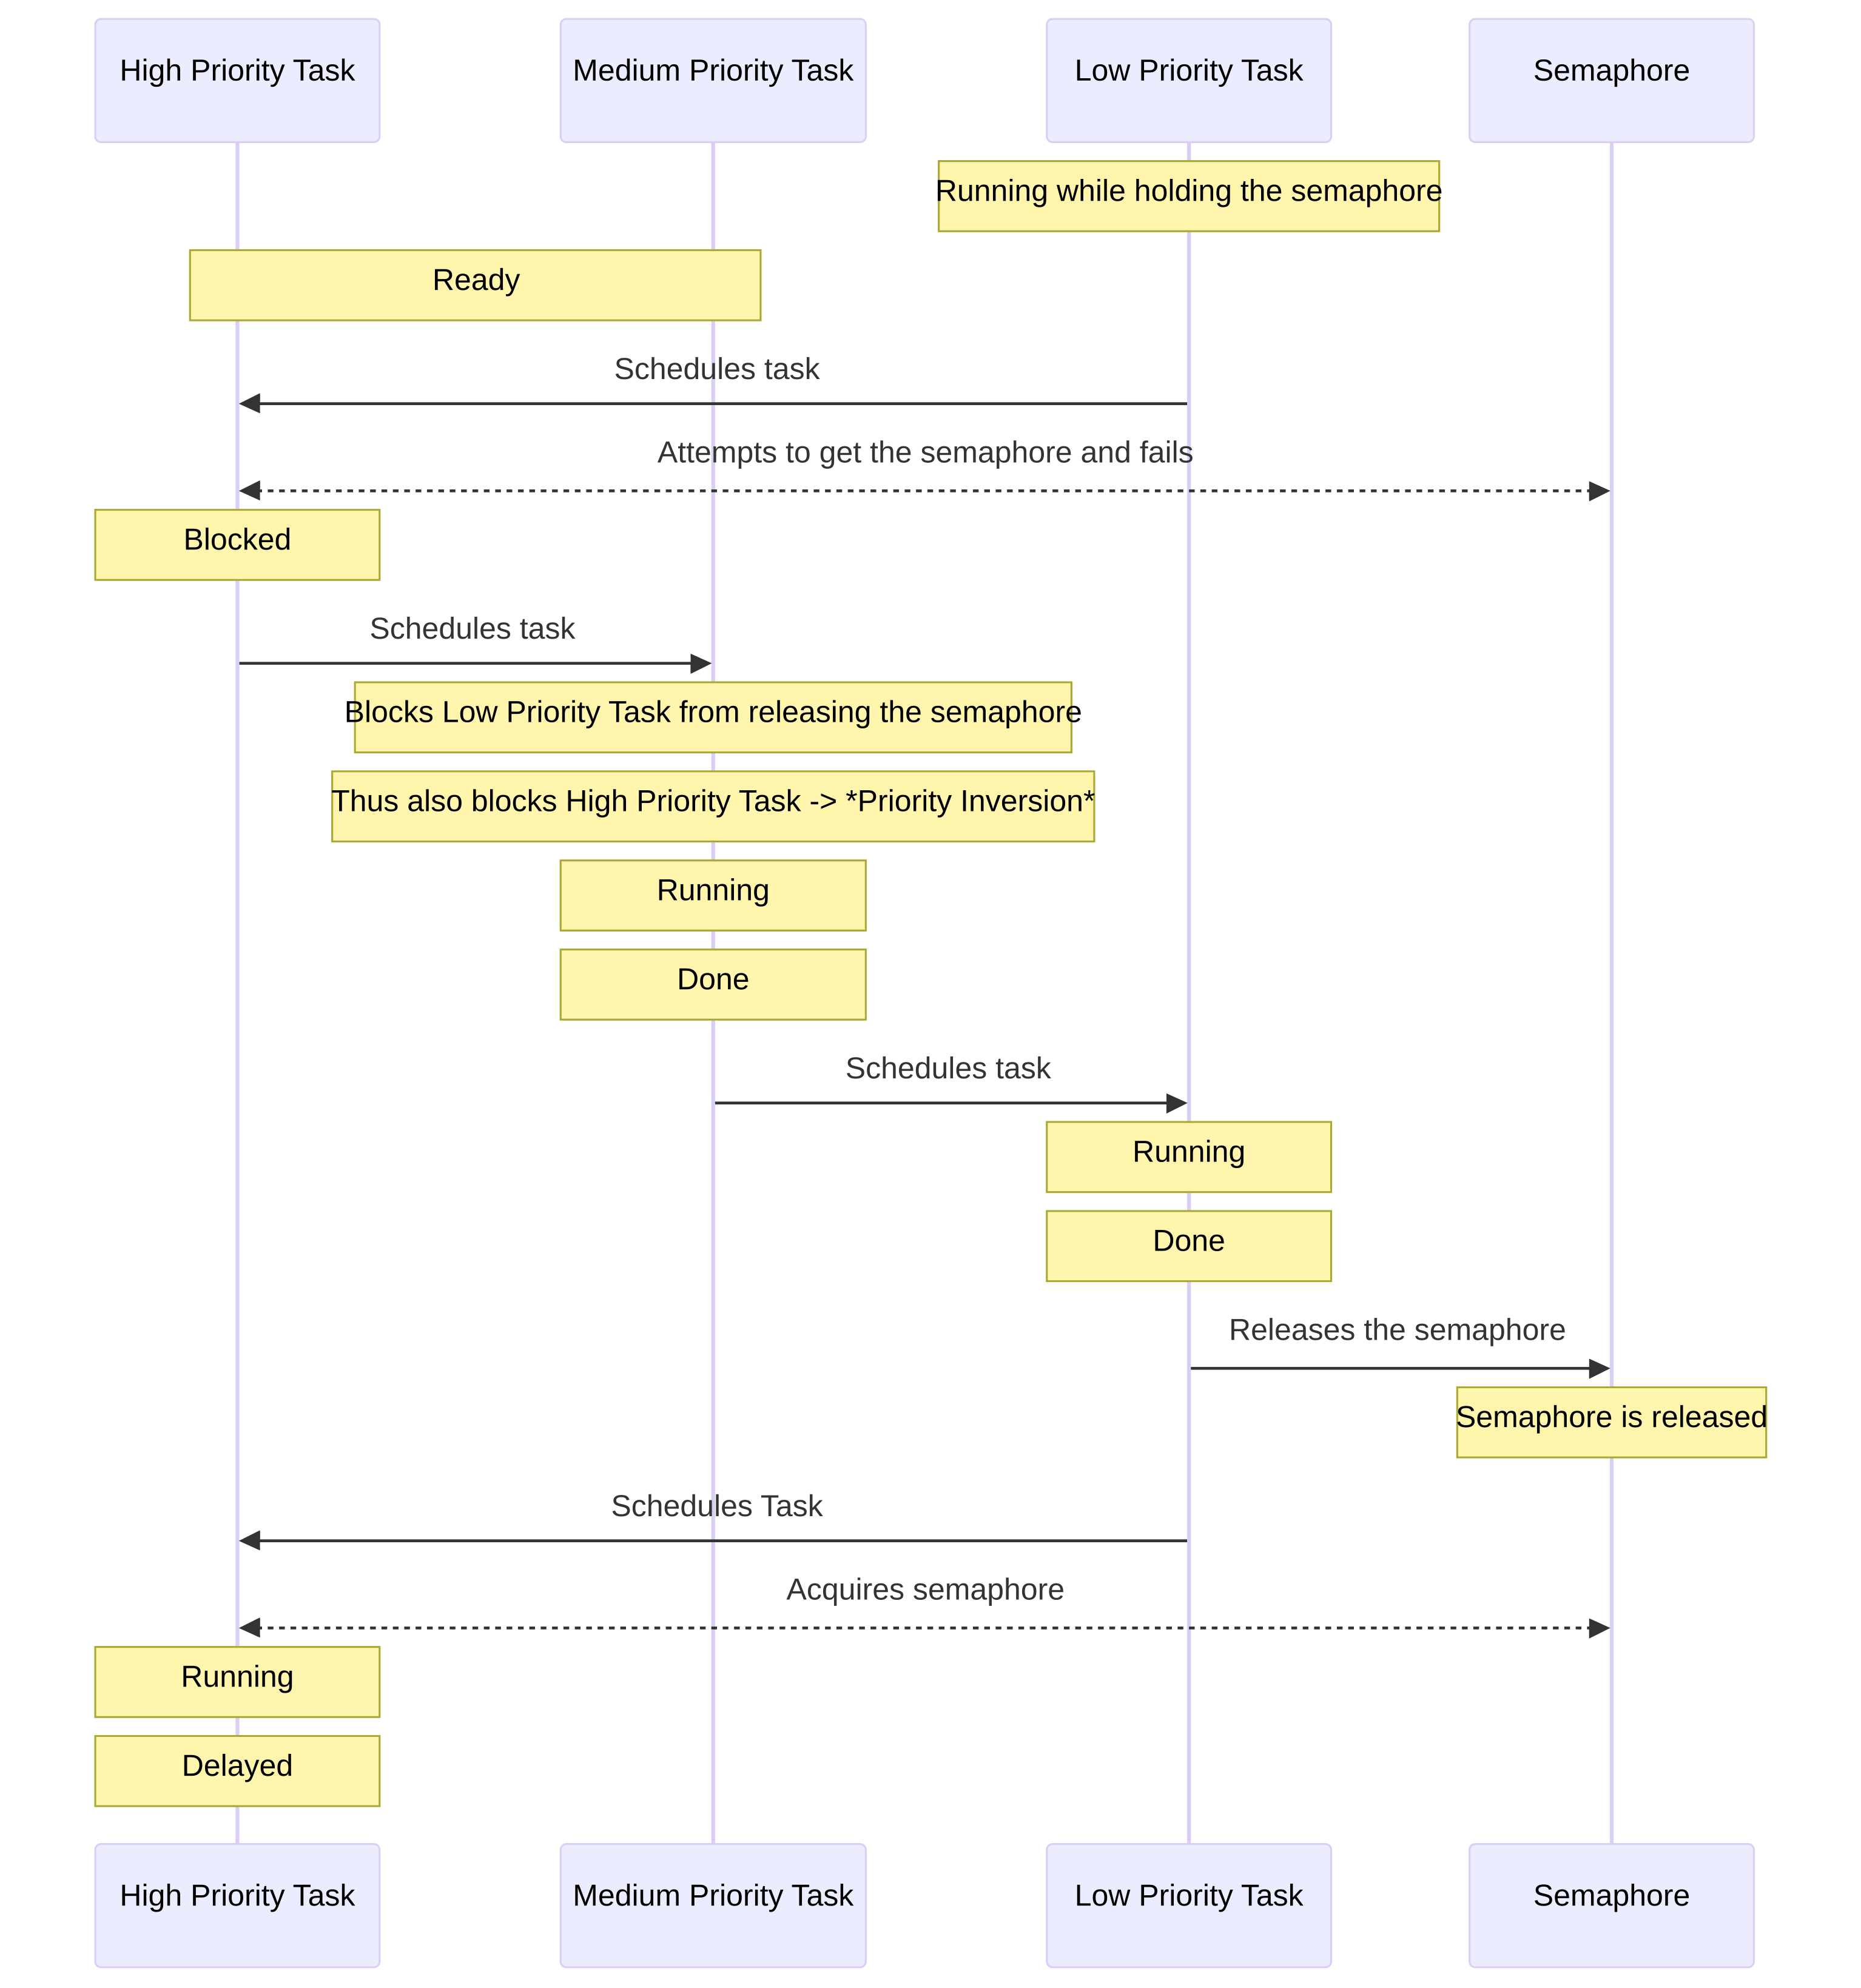
\includegraphics[width=1\textwidth]{assets/prio_inversion}
    \caption{Prioritätsinversion}
\end{figure}

\paragraph{Mutexe}

Im Gegensatz dazu sind Mutexe (Mutual Exclusion) Synchronisationsmechanismen,
die Prioritätsvererbung implementieren \cite{freertos_mutexes}. Wenn ein Task
auf einen Mutex wartet, der von einem niedriger priorisierten Task gehalten
wird, wird dieser Task temporär auf die Priorität des wartenden Tasks
erhöht~\cite{FreertosForumSemphMtx}, so dass er den Mutex und damit die von dem
watenden Task benötigte Ressource so schnell wie möglich wieder freigeben kann.

\begin{figure}[htb]
    \centering
    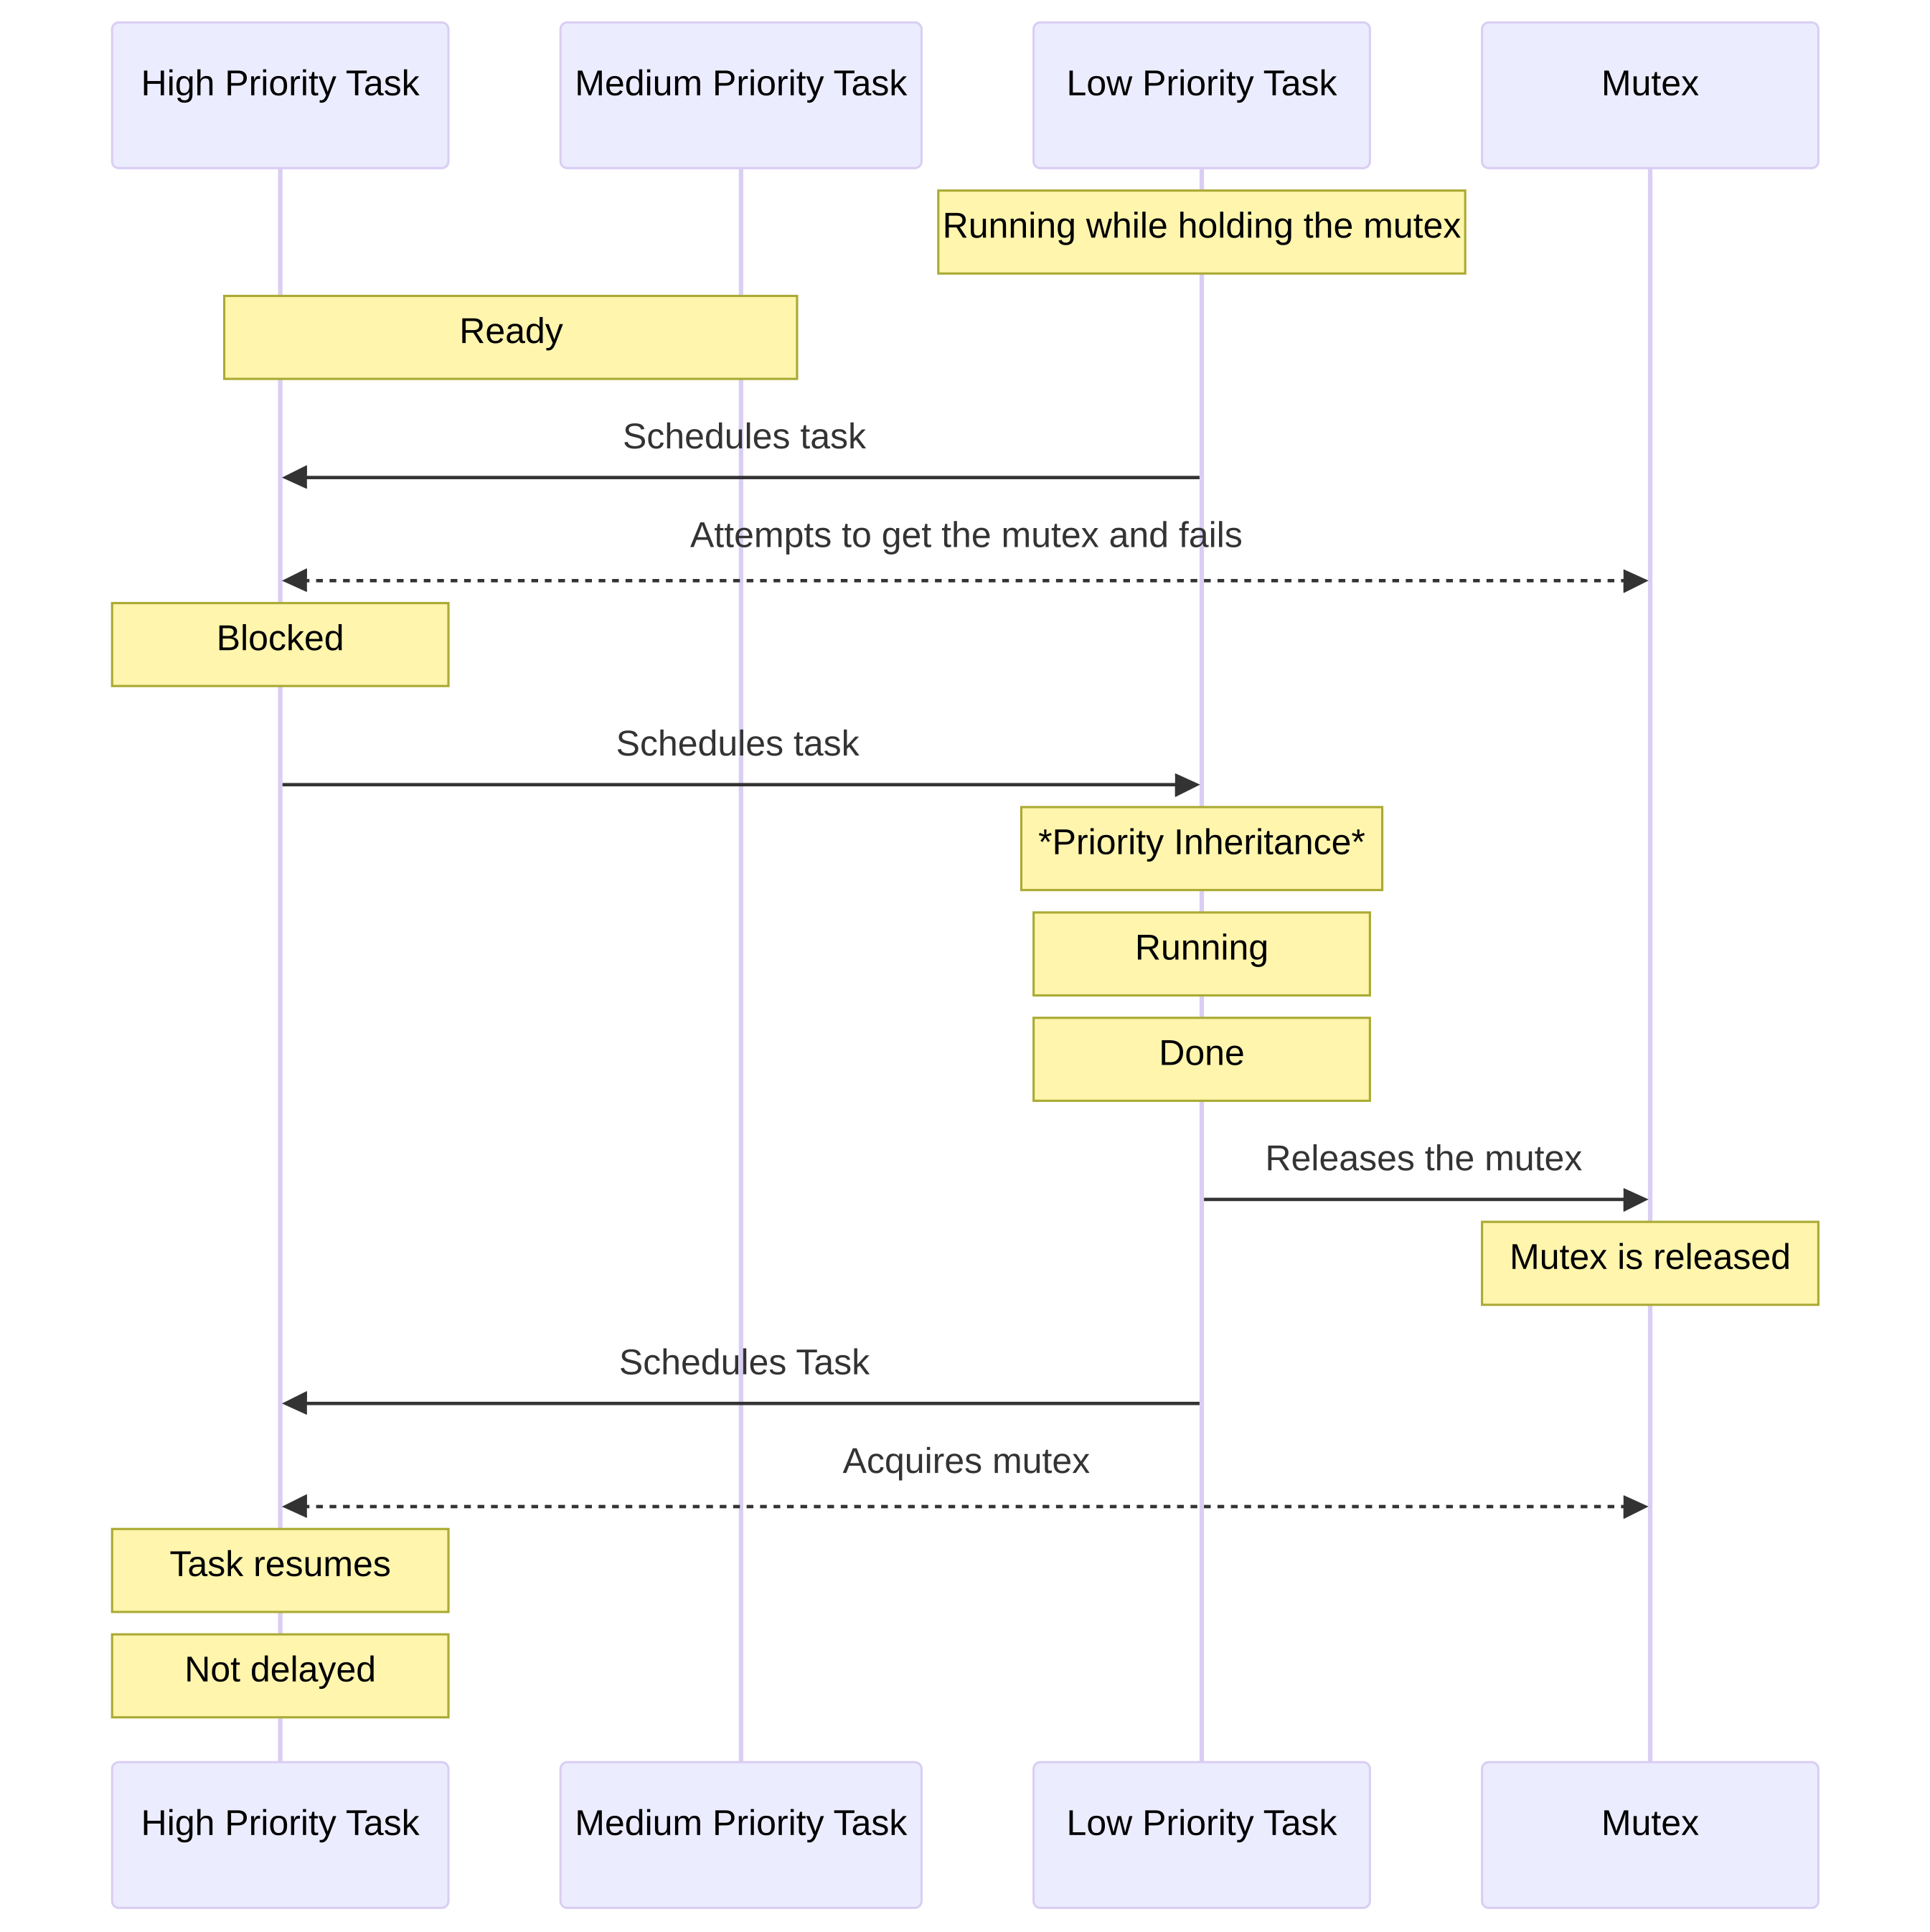
\includegraphics[width=1\textwidth]{assets/prio_inheritance}
    \caption{Prioritätsvererbung}
\end{figure}

\paragraph{Direct Task Notifications} \label{sec:direct_task_notification}

Direct Task Notifications sind ein effizienterer und ressourcenschonenderer
Mechanismus zur Task-Synchronisation \cite{freertos_task_notifications_desc}. Im
Gegensatz zu Semaphoren senden sie direkte Signale an einen Task, ohne die
zugrunde liegenden Queues zu benötigen, indem sie einfach einen internen Zähler
eines Tasks verändern \cite{freertos_tasks_c_213}. Analog zu Semaphoren wird
mittels Funktionen wie zum Beispiel \mintinline{c}|ulTaskNotifyGive()| dieser
Zähler inkrementiert~\cite{freertos_tasks_c_4296}, während Funktionen wie
\mintinline{c}|ulTaskNotifyTake()| ihn wieder
dekrementieren~\cite{freertos_tasks_c_3926}. Das Entblocken eines Tasks mittels
Direct Task Notifications soll bis zu 45\% schneller sein und benötigt weniger
RAM \cite{freertos_task_notifications_usage}.

\paragraph{Trace Hooks}

„Trace Hooks“ sind spezielle Macros von der FreeRTOS-API, deren Nutzung es
beispielsweise ermöglicht, Ereignisse im System zu verfolgen und zu
protokollieren. Diese Macros werden innerhalb von Interrupts beim Schedulen
aufgerufen und müssen immer vor der Einbindung von \mintinline{text}|FreeRTOS.h|
definiert werden \cite{freertos_rtos_trace_hooks}.

\subsection{Nutzung von Caches}

Caches sind schnelle Speicherkomponenten, die dazu dienen, Zugriffe auf häufig
verwendete Daten und Befehle zu beschleunigen und den Energieverbrauch zu
reduzieren \cite{ka001150}. In vielen modernen Mikrocontrollern, wie dem
Cortex-M7, ist der L1-Cache (Level 1 Cache) jeweils in einen Datencache
(D-Cache) und einen Instruktionscache (I-Cache) unterteilt \cite[S. 6]{an4667}.
Da der Zugriff auf den Hauptspeicher sowie auf den Flash generell viel langsamer
ist und mehrere Taktzyklen dauert~\cite{stm32_memory_sections}, können mit
L1-Caches 0-Waitstate-Zugriffe ermöglicht werden \cite[S. 6]{an4667}.

Der L1-Cache kann nur mit Speicherschnittstellen auf der \ac{AXI}-Busarchitektur
genutzt werden~\cite[S. 4]{an4839}. Hierzu zählen unter anderem der Flash, der
\ac{SRAM} sowie die beiden \ac{AHB}-Busse, die alle an den AXI-Bus angebunden
sind (siehe Abbildung \ref{fig:m7_sys_arch}).

\begin{figure}[htb]
    \centering
    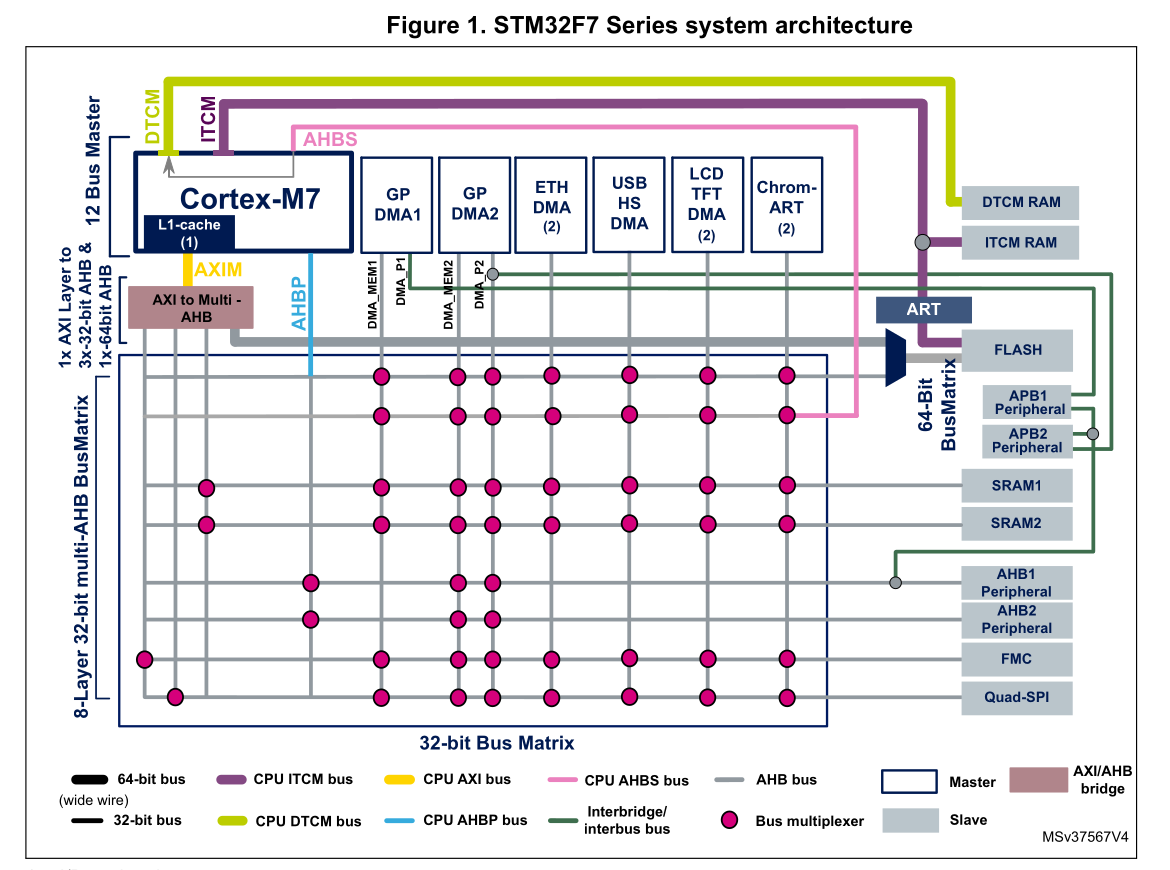
\includegraphics[width=1\textwidth]{assets/m7_system_arch}
    \caption{STM32F7 Systemarchitektur \cite[S. 9]{an4667}}
    \label{fig:m7_sys_arch}
\end{figure}

Aus der Matrix wird deutlich, dass für den Speicher zwischen SRAM und TCM-RAM
unterschieden wird. Die \ac{TCM} bietet niedrigere Zugriffszeiten als SRAM für
den Prozessor und ist nicht cachefähig. Während bei cachefähigem Speicher die
Zugriffszeit variiert (schnell aus dem Cache oder langsam aus dem externen
Speicher), ist die Zugriffszeit bei TCM konsistent und deterministisch. Dies
macht sie ideal für zeitkritische Routinen wie Interrupt-Handler oder
Echtzeitaufgaben. (\cite{arm_den0042})

Zusammenfassend lässt sich sagen, dass jeder normale, nicht gemeinsam genutzte
(non-shared) Speicherbereich gecacht werden kann, sofern er über das AXI-Bus
zugänglich ist \cite[S. 4]{an4839}~\cite[S. 7]{an4667}.

Aus der Tabelle für den internen Speicher wird deutlich, dass der Flash ab der
Adresse $0x0800 0000$ über das AHB-Bus angesprochen wird (siehe
\ref{fig:internal_mem_table}). Diese Adresse ist auch im Linker-Skript
standardmäßig für den Flash festgelegt. Daher kann der Instruktionscache über
den AXI-Bus für den Programm-Flash genutzt werden.

\begin{figure}[htb]
    \centering
    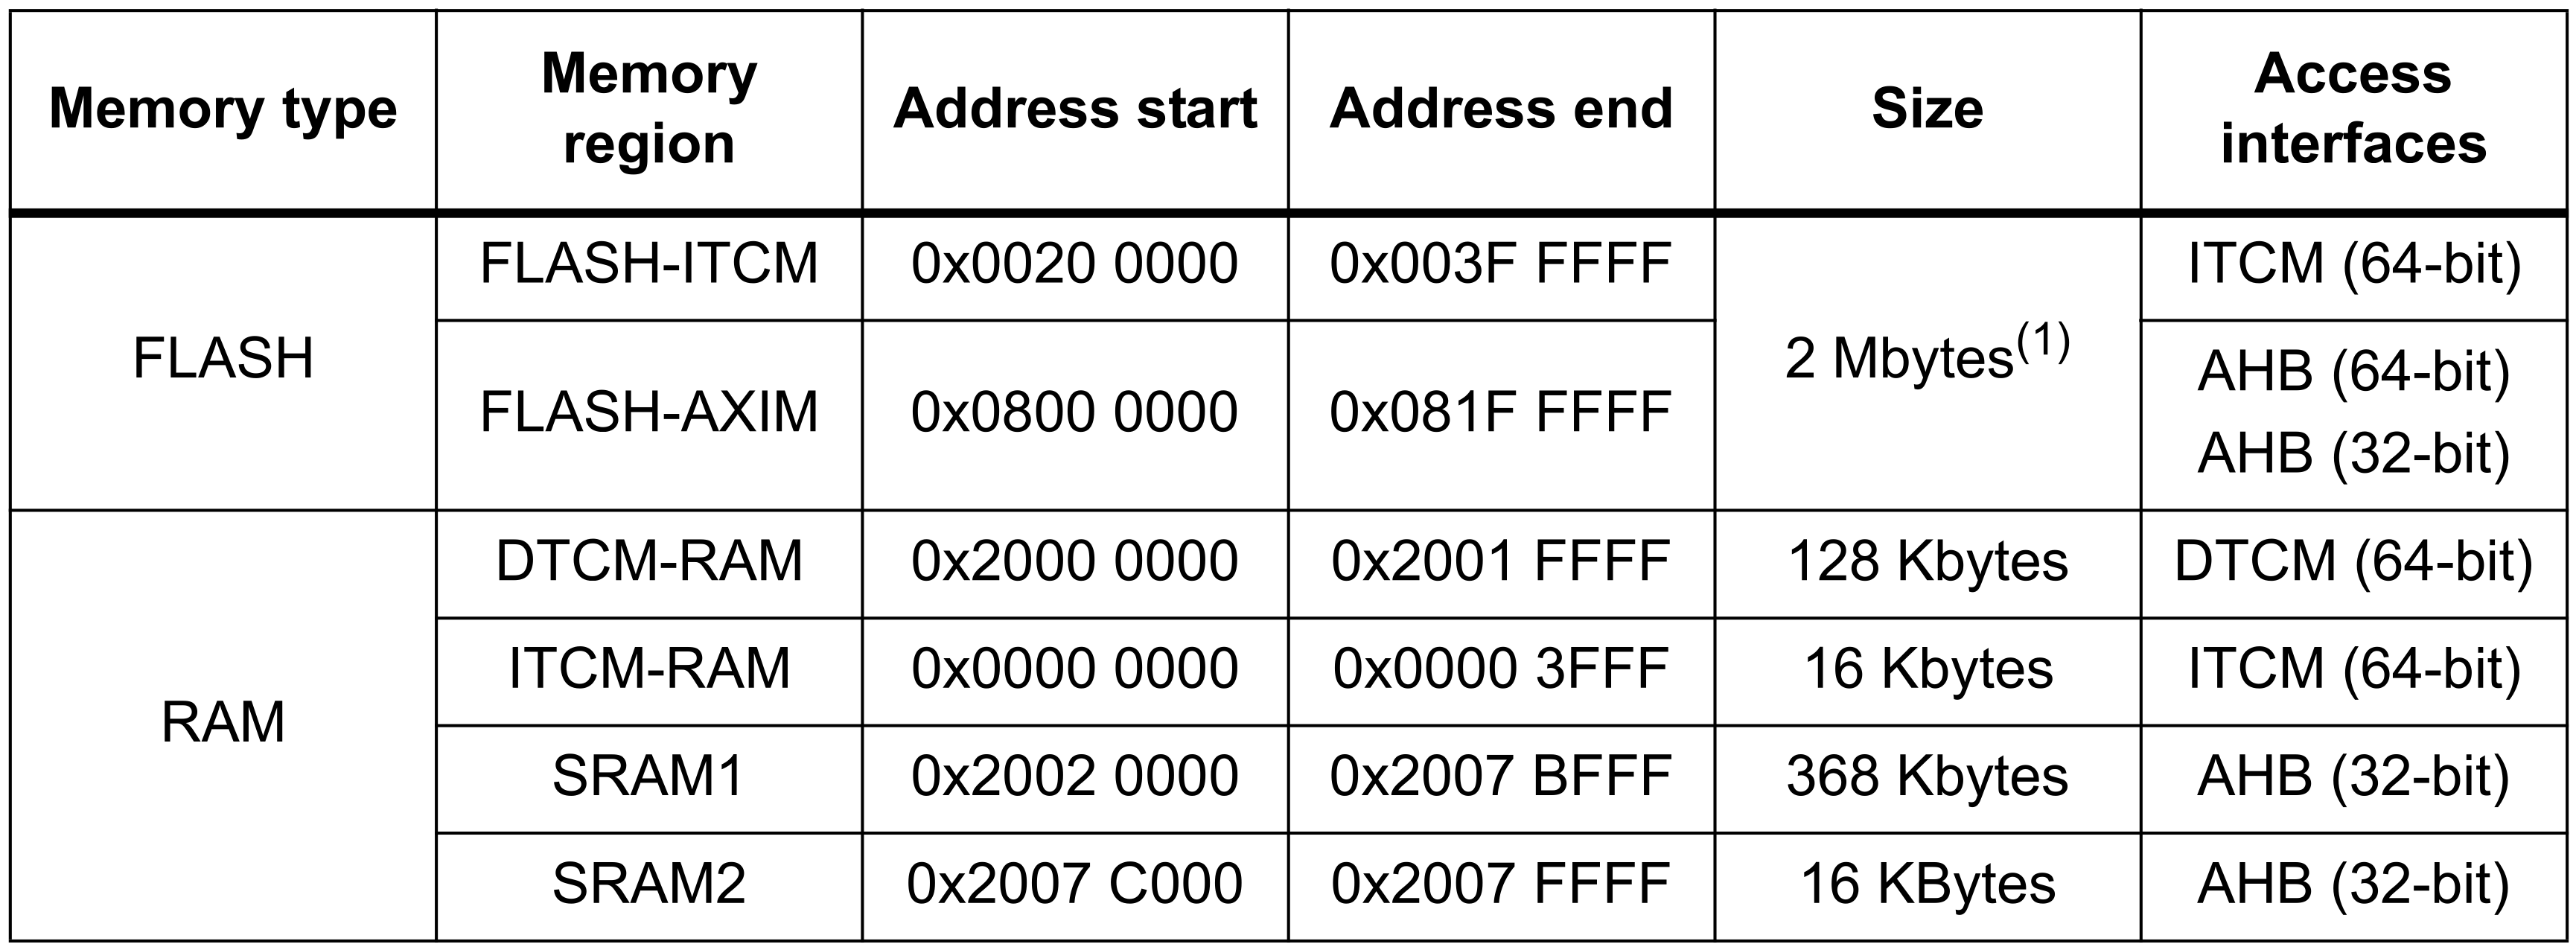
\includegraphics[width=1\textwidth]{assets/internal_mem_table}
    \caption{STM32F7 Systemarchitektur \cite[S. 14]{an4667}}
    \label{fig:internal_mem_table}
\end{figure}

\begin{code}
\begin{minted}{c}
MEMORY
{
RAM (xrw)      : ORIGIN = 0x20000000, LENGTH = 512K
FLASH (rx)      : ORIGIN = 0x8000000, LENGTH = 2048K
}
\end{minted}
    \captionof{listing}{Definition Speicherbereich im Linker-Script für STM32F7}
\end{code}

Um Caches zu nutzen, bietet die STM-\ac{HAL} dedizierte Funktionsaufrufe in der
API an \cite[S. 4]{an4839}:

\begin{code}
\begin{minted}{c}
void SCB_EnableICache(void)
void SCB_EnableDCache(void)
void SCB_DisableICache(void)
void SCB_DisableDCache(void)
void SCB_InvalidateICache(void)
void SCB_InvalidateDCache(void)
void SCB_CleanDCache(void)
void SCB_CleanInvalidateDCache(void)
\end{minted}
    \captionof{listing}{Cache-Funktionen}
\end{code}

Bei einer Cache-Clean-Operation werden modifizierte Cache-Zeilen (Dirty Cache
Lines), die durch das Programm aktualisiert wurden, zurück in den Hauptspeicher
geschrieben \cite[S. 4]{an4839}. Dieser Vorgang wird gelegentlich auch als
„flush” bezeichnet. Eine Cache-Invalidierungsoperation markiert den Inhalt des
Caches als ungültig, sodass bei einem erneuten Zugriff auf dieselben Daten der
Speicher neu ausgelesen und der Cache aktualisiert werden muss.

Allerdings kann beim Aktivieren von Caches für Speicherbereiche, die vom
DMA-Controller genutzt werden, ein Problem der Cache-Kohärenz (Cache Coherency)
entstehen, da der Prozessor in diesem Fall nicht der einzige Master ist, der auf
diese Speicherbereiche schreibt und liest. Daher sind Operationen wie
Cache-Clean und Cache-Invalidierung essentiell, um die Konsistenz zwischen Cache
und Speicher sicherzustellen.

\subsubsection{Cache-Clean bei DMA} \label{sec:cache_clean}

Damit der DMA-Controller stets auf aktuelle Daten zugreifen kann, ist eine
Cache-Clean nach jeder Datenmodifikation erforderlich. Sie stellt sicher, dass
die Daten nicht nur im Cache modifiziert, sondern auch noch zurück in den
Speicher geschrieben werden \cite[S. 6]{an4839}. Ohne diesen Schritt würden die
Änderungen nicht im SRAM widergespiegelt, und der DMA-Controller würde weiterhin
veraltete Daten verwenden.

\subsubsection{Cache-Invalidierung bei DMA}

Bei Daten, die aus Speicherbereichen gelesen werden, auf die auch der
DMA-Controller zugreift, muss zuvor eine Cache-Invalidierung erfolgen
\cite{embeddedexpert_cache}. Dies garantiert, dass die Daten immer direkt aus
dem RAM gelesen werden. Da der DMA-Controller die Daten jederzeit ändern kann,
sind die gecachten Daten per se ungültig und müssen durch eine Aktualisierung
ersetzt werden.

\subsection{Methode zur Echtzeitanalyse}

Um die Echtzeitanalyse der Steuerungssoftware durchzuführen, ist eine Methode
erforderlich, mit der beliebige Ausführungsabschnitte der Software flexibel,
präzise und threadsicher gemessen werden können. Da die Software multithreaded
ist, muss ebenfalls sichergestellt werden, dass die Messungen trotz preemptivem
Scheduling sowie Interrupts korrekt und zyklengetreu durchgeführt werden können.

Basierend auf den oben genannten Herausforderungen bietet die \ac{DWT} als eine
geeignete Lösung \cite{ARM_KA001499}. Die DWT ist ein Debug-Einheit in
Prozessoren inklusive ARMv7-M \cite{ARMv7_ref_man_dwt_about}, die das Profiling
mittels Zähler unterstützen \cite{ARMv7_ref_man_dwt_profiling}. Ein für diese
Arbeit zentraler Teil der DWT ist der Zyklenzähler \mintinline{c}|DWT_CYCCNT|,
der bei jedem Takt inkrementiert wird, solange sich der Prozessor nicht im
Debug-Zustand befindet \cite{ARMv7_ref_man_dwt_cycle}. Dadurch ermöglicht die
DWT beispielsweise die Erfassung von Echtzeitaspekten mit zyklengenauer
Präzision under normaler Operation \cite{ARMv7_ref_man_dwt}.

\subsubsection{Beispiel: SEGGER SystemView}

Ein Beispiel hierfür ist SEGGER SystemView, ein Echtzeit-Analysewerkzeug, das
die DWT einsetzt, um Live-Code-Profiling auf eingebetteten Systemen
durchzuführen \cite{SEGGER_SystemView}.

Das SEGGER SystemView nutzt den DWT-Zyklenzähler, indem die Funktion \linebreak
\mintinline{c}|SEGGER_SYSVIEW_GET_TIMESTAMP()| für Cortex-M3/4/7-Prozessoren
einfach die hardkodierte Registeradresse des Zyklenzählers zurückgibt \cite[S.
65]{Segger_SystemView_manual}\cite{Arm_DWT_Programmers_Model}, anstatt die
interne Funktion \mintinline{c}|SEGGER_SYSVIEW_X_GetTimestamp()| aufzurufen.
